%%%%%%%%%%%%%%%%%%%%%%%%%%%%%%%%%%%%%%%%%%%%%%%%%%%%%%%%%%%%%%%%%%%%%
% HEADERS AND PACKAGES
%%%%%%%%%%%%%%%%%%%%%%%%%%%%%%%%%%%%%%%%%%%%%%%%%%%%%%%%%%%%%%%%%%%%%

\documentclass[11pt]{article}
\usepackage[T1]{fontenc}
\usepackage{lmodern,textcomp}
\usepackage{adjustbox}
\usepackage{helvet}
\usepackage{natbib}
\usepackage{bibentry}
\usepackage[american]{babel}
\usepackage{graphicx}
\usepackage{hhline}
\usepackage{multirow}
\usepackage{hyperref}
\usepackage{times}
\usepackage{amsmath}
%\usepackage{csquotes}% Recommended
\usepackage{amssymb}
\usepackage{longtable}
\usepackage{rotating}
\usepackage{tikz}
\usepackage{relsize}
\usepackage{xcolor}
\usepackage{array}
\usepackage{authblk}
\usepackage{booktabs}
\usepackage{float}
\usepackage{url}
\usepackage{caption}
\usepackage{subcaption}
\usepackage{algorithm}
\usepackage{algorithmic}
\usepackage{longtable}
\usepackage{framed}
%\usepackage[ruled, linesnumbered]{algorithm2e}
\usepackage{makecell}
\usepackage{mathtools}

\DeclarePairedDelimiter\ceil{\lceil}{\rceil}
\DeclarePairedDelimiter\floor{\lfloor}{\rfloor}



%%%%%%%%%%%%%%%%%%%%%%%%%%%%%%%%%%%%%%%%%%%%%%%%%%%%%%%%%%%%%%%%%%%%%
% DRAWINGS
%%%%%%%%%%%%%%%%%%%%%%%%%%%%%%%%%%%%%%%%%%%%%%%%%%%%%%%%%%%%%%%%%%%%%

\usepackage{tikz}
\usepackage{forest}

%%%%%%%%%%%%%%%%%%%%%%%%%%%%%%%%%%%%%%%%%%%%%%%%%%%%%%%%%%%%%%%%%%%%%
% THEOREMS
%%%%%%%%%%%%%%%%%%%%%%%%%%%%%%%%%%%%%%%%%%%%%%%%%%%%%%%%%%%%%%%%%%%%%

\newtheorem{theorem}{Theorem}
\newtheorem{assumption}{Assumption}
\newtheorem{problem}{Problem}
\newtheorem{remark}{Remark}
\newtheorem{corollary}{Corollary}
\newtheorem{definition}{Definition}
\newtheorem{proposition}{Proposition}
\newtheorem{lemma}{Lemma}
\newtheorem{example}{Example}


%%%%%%%%%%%%%%%%%%%%%%%%%%%%%%%%%%%%%%%%%%%%%%%%%%%%%%%%%%%%%%%%%%%%%
% EQUATIONS
%%%%%%%%%%%%%%%%%%%%%%%%%%%%%%%%%%%%%%%%%%%%%%%%%%%%%%%%%%%%%%%%%%%%%

\newcommand{\overrideeqlabel}[1]{\renewcommand{\theequation}{#1}}
\newcommand{\reseteqlabel}{\addtocounter{equation}{-1}%
\renewcommand{\theequation}{\arabic{chapter}.\arabic{equation}}}
\newenvironment{eqwithlabel}[1]{\overrideeqlabel{#1}\begin{equation}}%
{\end{equation}\reseteqlabel}

%%%%%%%%%%%%%%%%%%%%%%%%%%%%%%%%%%%%%%%%%%%%%%%%%%%%%%%%%%%%%%%%%%%%%
% PAGE SETUP
%%%%%%%%%%%%%%%%%%%%%%%%%%%%%%%%%%%%%%%%%%%%%%%%%%%%%%%%%%%%%%%%%%%%%

%\usepackage[a4paper,outer=2cm,inner=2cm,top=2cm,bottom=2cm,marginparwidth=4cm,marginparsep=0.5cm]{geometry}
\usepackage[a4paper,outer=2cm,inner=2cm,top=2cm,bottom=2cm,marginparwidth=0cm,marginparsep=0cm]{geometry}
\usepackage{setspace}
%\doublespacing
\newcommand{\liner}{\underline{${}_{}$\hspace{\textwidth}}\hspace{-\textwidth}}
\newcommand{\linel}{\hfill\hspace{-\textwidth}\underline{${}_{}$\hspace{\textwidth}}}
\newcommand{\markpages}[1]{\markboth{\hspace*{0.1cm} #1 \hfill \linel}{\liner #1 \hspace*{0.1cm}}}


%%%%%%%%%%%%%%%%%%%%%%%%%%%%%%%%%%%%%%%%%%%%%%%%%%%%%%%%%%%%%%%%%%%%%
% COLORS
%%%%%%%%%%%%%%%%%%%%%%%%%%%%%%%%%%%%%%%%%%%%%%%%%%%%%%%%%%%%%%%%%%%%%
\definecolor{marcella}{rgb}{0.0,0.0,0.0} %What Marcella has changed
\def\marcella{\textcolor{marcella}}
\definecolor{bobby}{rgb}{0.0,0.0,0.0} %What Bobby has changed
\def\juergen{\textcolor{bobby}}
\definecolor{andre}{rgb}{0.0,0.0,0.0} %What Andre has changed
\def\hallo{\textcolor{andre}}


%%%%%%%%%%%%%%%%%%%%%%%%%%%%%%%%%%%%%%%%%%%%%%%%%%%%%%%%%%%%%%%%%%%%%
% SETTINGS
%%%%%%%%%%%%%%%%%%%%%%%%%%%%%%%%%%%%%%%%%%%%%%%%%%%%%%%%%%%%%%%%%%%%%

\selectlanguage{american}
\urlstyle{same}

%%%%%%%%%%%%%%%%%%%%%%%%%%%%%%%%%%%%%%%%%%%%%%%%%%%%%%%%%%%%%%%%%%%%%
% TITLEPAGE
%%%%%%%%%%%%%%%%%%%%%%%%%%%%%%%%%%%%%%%%%%%%%%%%%%%%%%%%%%%%%%%%%%%%%

\title{Modelling dynamic electric vehicle routing problem with heterogeneity and uncertainty}
\author{ }
\date{}

%%%%%%%%%%%%%%%%%%%%%%%%%%%%%%%%%%%%%%%%%%%%%%%%%%%%%%%%%%%%%%%%%%%%%
% BEGIN DOCUMENT
%%%%%%%%%%%%%%%%%%%%%%%%%%%%%%%%%%%%%%%%%%%%%%%%%%%%%%%%%%%%%%%%%%%%%

%%%%%%%%%%%%%%%%%%%%%%%%%%%%%%%%%%%%%%%%%%%%%%%%%%%%%%%%%%%%%%%%%%%%%%%%%%%%%%%%
\begin{document}
%%%%%%%%%%%%%%%%%%%%%%%%%%%%%%%%%%%%%%%%%%%%%%%%%%%%%%%%%%%%%%%%%%%%%%%%%%%%%%%%

\maketitle

\begin{abstract}
	With more and more serious issues like air pollution and traffic noise in transport sector, a fast growing number of electric vehicles has been used for various purpose in road transport, including urban freight transport. To promote the usage of electric vehicle in urban freight transport, this study investigates the dynamic vehicle routing problem with consideration of heterogeneous vehicle types and mixed-type charging facilities, as well as multiple uncertain factors in real operation. It is a challenge to incorporate charging activity into the route plan since the availability of charging station and the travel time en-route are stochastic. The decision-maker needs to assign the right vehicle type to a certain route with minimized total time to implement the routing plan. An adaptive solution approach based on multiple scenario approach and two heuristics is developed to solve the proposed model. To validate the proposed model and test the solution approach, multiple numerical experiments are conducted based on a benchmark dataset.
\end{abstract}
\textbf{Keywords} Electric vehicle routing problem, Heterogeneous electric vehicles, Mixed-type charging, Uncertainty, Dynamic approach, Multiple scenario approach


%%%%%%%%%%%%%%%%%%%%%%%%%%%%%%%%%%%%%%%%%%%%%%%%%%%%%%%%%%%%%%%%%%%%%%%%%%%%%%%%
\section{Introduction}
%%%%%%%%%%%%%%%%%%%%%%%%%%%%%%%%%%%%%%%%%%%%%%%%%%%%%%%%%%%%%%%%%%%%%%%%%%%%%%%%

Although road urban freight transport may cause various issues, such as traffic congestion, traffic noise, air pollution, energy consumption, and high logistics costs, it remains the primary mode of urban freight transport. The use of electric vehicles (EVs) has emerged as a promising solution to reducing such environmental and sustainable concerns. Its is evident that EVs operate more silently than conventional vehicles, and they could help reduce traffic emission significantly.  Nevertheless, how to run EVs efficiently and economically under various features and limitations associated with EV, for instance, limited driving range, limited load capacity, long charging time and the scarcity of charging station (CS), is a challenge to be addressed before EVs can be used for freight transport widely.

To promote the integration and operation of EVs to freight transport, several models of electric vehicle routing problem (EVRP) have been proposed during the past few years. As optimization decision models seek to represent real-life problems, research on EVRP has introduced several variants. One of them is the heterogeneous EVRP (HEVRP). Logistics companies usually hold a fleet of diverse EVs with different acquisition cost, capacity, driving range, and energy consumption. Therefore, fleet management, i.e. selecting the right EV for a certain transportation request, is highly important. In HEVRP, it is considered that EVs differ in their capacity, battery size, and purchasing cost. Another variant of the EVRP is the stochastic EVRP (SEVRP). In real life, one or more inputs of the problem are often uncertain, and the developments in the area of algorithms and the area of information technologies, e.g. development of intelligent transportation systems (ITS), have rendered possible to freight providers the use of real-time data on the management of their operations. 

That is, VRP can now be solved dynamically, i.e. on real-time manner....

we consider the possibility of performing a partial recharge at a station. This implies that for each vehicle we have to decide where and when to recharge, but also how much....

However, since solving it to optimality for realistic sized instances is prohibitive, we decided to focus on heuristic approaches.....

While the vehi- cle is traveling, the battery charge level decreases proportionally with the distance traversed and the vehicle may need to visit a recharging station in order to continue its route. The battery is recharged at any quantity and the duration of the recharge depends on the initial state of battery charge....

This waiting time varies depending on the time of the day because some time periods are more crowded due to rush hours and the demand is higher during these periods...

Many different heuristics have been successfully applied to vehicle routing problems with additional constraints, providing near optimal solutions within a short computational time....

The experiments have focused on evaluating the per- formance of the proposed algorithms and analyzing some of the main characteristics of the problems considered, mainly regarding the size and geographical configuration of the instances, the number of recharge stations, the use of multiple tech- nologies and partial recharges and the autonomy of the vehicles.....

explain that there might not be enough time to compute solutions

Although a diversity of EVRP models have been proposed with consideration of various factors and constraints, several key factors associated with EVs are missing, and more importantly the relationship among various factors lacks exploration. 

In this paper, we introduce a model for the dynamic heterogeneous electric vehicle routing problem (DHEVRP) with consideration of heterogeneity and uncertainty. This model aims to address multiple challenges associated with EV operation in an adaptive way, i.e. sequential decision-making. Heterogeneity comes from multiple types of EVs with different loading capacity, battery capacity and energy consumption, as well as various charging rates at different CSs. Three sources of uncertainty are considered: travel time, charging station availability, and waiting time at a CS. Travel time is considered stochastic due to traffic congestion. For example, travel time is usually larger at peak hours than at non-peak hours along the same route. We assume that each CS has a probability of being available, and in case of CS is fully occupied, a stochastic waiting time will be imposed for the EV in queue. Moreover, both time window and service time are considered for each customer. Penalty cost/time will be charged if delivery occurs out of the time window. The objective function of the DHEVRP consists of en-route time and on-demand charging time. En-route includes travel time, service time, and penalty cost/time for early or late delivery whereas on-demand charging time is a function of availability of CS, waiting time at CS, charging rate, remaining and expected battery levels. To solve this problem, we proposed a dynamic solution method in which the time horizon is divided into intervals. The goal is to design a solution for how to serve customers and when/where recharge the EV within the next time interval, using both deterministic and stochastic information about the inputs.

To our best knowledge, it is the first study to consider both heterogeneous EVs and stochasticity in EVRP, and both considerations are quite practical and important in real-life EVRP. In the literature, most parameters in EVRP were either given as fixed or considered as stochastic and separate from each other. In this study, we aim to explore the connection among multiple parameters to develop interlinked conditions. For example, in our proposed model, we consider charging time as a function of a series of parameters, like remaining battery level, charging rate, and so on. Rather than fully charged setting in most studies, we consider on-demand charging, i.e. top-up charges, based on the adaptive route plan, which makes the charging strategy more flexible and economical. Last but not the least, different cases will be tested based on benchmark networks to validate the DEHVRP model and prove the efficiency of the proposed solution method.

The structure of the paper is as follows. In the next section, a review research on EVRP is briefly presented. In Section~\ref{section:model}, the mathematical formulation of the problem is shown. The proposed solution approach is introduced in Section ~\ref{section:approach} followed by the description of the dataset in Section~\ref{section:dataset}. In Section~\ref{section:cases}, we define the different cases used in the experiments. The computational results are displayed in Section~\ref{section:results}, and the work is concluded in Section~\ref{section:conclusion}.

%%%%%%%%%%%%%%%%%%%%%%%%%%%%%%%%%%%%%%%%%%%%%%%%%%%%%%%%%%%%%%%%%%%%%%%%%%%%%%%%
\section{Literature Review}
%%%%%%%%%%%%%%%%%%%%%%%%%%%%%%%%%%%%%%%%%%%%%%%%%%%%%%%%%%%%%%%%%%%%%%%%%%%%%%%%
In this work, we cover two categories of the electric vehicle routing problem. A brief description of these classes together with examples of works that have investigated them are presented as follows. 

The first class is the HEVRP. Companies usually hold a fleet of diverse electric vehicles regards to, for instance, driving range. The fleet management, i.e. selecting the right EV for a certain transportation request, is highly important when the fleet of electric vehicles is heterogeneous. This class of EVRP has been proposed to represent this situation. The HEVRP may, therefore, include many types of electric vehicles which can differ in capacity, battery capacity, energy battery consumption, charge level, and fixed cost. To the best of our knowledge only \cite{Hiermann2016}, \cite{Penha2016}, \cite{Jie2019}, and \cite{Kopfer2019} have approached the HEVRP. \cite{Hiermann2016} and \cite{Penha2016} studied the electric fleet size and mix vehicle routing problem with time windows and recharging stations (E-FSMFTW). In this problem, each customer has a specific demand, a duration of the service, and must be serviced within its time window. It was assumed that the EVs vary in their transportation capacity, battery size, and purchasing costs. \cite{Jie2019} introduced the two-echelon capacitated electric vehicle routing problem with battery swapping stations (2E-EVRP-BSS) with heterogeneous EVs in different echelons. In this problem, the freight available in a depot (echelon) is transported to the transfer stations (echelon) by large EVs, and then small EVs are used to deliver the freight to the customers. The EVs operating in the different echelons have different load capacity and battery driving ranges. \cite{Kopfer2019} introduced the energy vehicle routing problem with time windows, recharge stations and vehicle classes (EVRPTW-R-VC), where the use of a heterogeneous fleet composed of differently sized EVs and combustion-powered vehicles (CVs) is investigated. 

The second class is the SEVRP. In contrast to the assumptions of the classical EVRP, in the real world one or more of the elements of the EVRP are uncertain. The inputs of the EVRP that have been assumed to be stochastic are customer presence \citep{Shi2019}, demands \citep{Lu2019}, travel time \citep{Shao2017, Bi2019, Reyes2019}, and energy consumption \citep{Pelletier2019}. Because of the importance of the time frame in the decision-making process, the SEVRP can be examined from two perspectives: static or dynamic. From a static perspective, the goal is to calculate a robust a-priori solution that undergoes minor changes during its execution to manage the fluctuations in the uncertain inputs. From a dynamic perspective, the aim is to design a route plan in an online way reporting to every vehicle what to do next. For this reason, the SEVRP can be classified either as static and stochastic EVRP (SSEVRP) or dynamic and stochastic EVRP (DSEVRP). In the SSEVRP, decisions are made at the planning phase and define actions which are implement at the execution phase, whereas in the DSEVRP decisions are made as soon as a new event occurs. In the latter, route plans are reoptimised at predefined stages with respect to both the current condition of the system and the available stochastic information. \cite{Pelletier2019} and \cite{Reyes2019} approached the SEVRP with a static strategy. Although in both studies the term robust refers to guaranteeing that no EV will run out of battery during the execution of its route, \cite{Pelletier2019} proposed a robust optimisation framework to the electric vehicle routing problem with energy consumption uncertainty (EVRP-ECU), while \cite{Reyes2019} introduced a hybrid solution approach to the electric vehicle routing problem with stochastic travel times (EVRPST). \cite{Shao2017}, \cite{Lu2019} and \cite{Bi2019} have investigated the stochastic EVRP from a dynamic perspective. \cite{Shao2017} introduced a solution method that integrated a dynamic Dijkstra algorithm with a genetic algorithm (GA) to solve the electric vehicle routing problem with charging time and variable travel time (EVRP-CTVTT). \cite{Lu2019} approached the dynamic capacitated electric vehicle routing problem (DCEVRP) with stochastic customers and stochastic demands by transforming the problem into a series of static problems. For solving the series of static problems, they introduced a bi-strategy based optimization algorithm (BSOA). \cite{Bi2019} considered the dynamic electric vehicle routing problem with battery charging and discharging and stochastic travel time and stochastic demands. The authors designed a markov decision process (MDP) model which incorporates an analytical battery model to better capture the discharging and charging pattern of the EVs. To solve this model, a hybrid rollout algorithm (HRA) which combines a pre-planning strategy and a rollout algorithm was developed.

In this work, we combine the two classes of EVRP described before and introduce the DHEVRP. Therefore, in this model, different types of EV are available and uncertainties are present, and the problem is solved using a dynamic approach. The EVs differ based on capacity, battery capacity, energy battery consumption, and charging rate. The sources of uncertainty are: travel time, charging station availability, and waiting time at a CS. Stochastic charging station availability means that each CS has a probability of being available. If the CS is available, the EV is promptly recharged, otherwise stochastic waiting time will be imposed. On-demand charging time is defined as the whole period an EV remains at the CS, and it is considered as a function of the parameters: availability of CS, waiting time at CS, energy consumption rate, charging rate, remaining and target battery level. The remaining battery level is calculated based on the initial battery level and en-route energy consumption. The latter is a function of the travel distance and energy consumption rate. The target battery level of an EV is determined based on the estimation of energy consumption on the remainder of its route. That is to say, instead of recharging the battery from empty-to-full, top-up charging are done. The battery is charged to a level so that the EV is able to attend the remaining customers and return to the depot. Historical data on the stochastic inputs is available, and the decision-making process is divided into several stages. The first stage is called planning stage. In this stage, we use the stochastic information about the inputs to calculate the so-called a-priori route plan. After that, the a-priori route plan is reoptimised every time a new event occurs. An event happens when the true value of any of the stochastic inputs is disclosed. Figure \ref{Fig1} illustrates the difference between the stages for a single EV (route) when the true values of the stochastic travel times are revealed. At the beginning of a work day ($t = 0$), an EV starts to execute its route in accordance to the a priori route plan (represented in gray). The a priori route plan was designed in the previous day considering the known inputs, e.g. customers' locations, and the expected values of the uncertain inputs. In the next stage ($t = t_e$), the battery energy is consumed as the EV follows its route. Based on the a priori route plan, the EV should consume one unit of battery power as it travels from depot to customer 1 and one unit from customer 1 to customer 2. Although the traffic was normal (black arrow), i.e. normal travel time, and one unit of battery was thus used from depot to customer 1, the traffic was congested (red arrow), i.e. higher travel time, from customer 1 to customer 2 and two units of battery were used by the EV. Therefore, instead of being charged after attending customer 3 as planned in the a priori route plan, the EV must move to a different CS right after serving customer 2. Once all the stochastic travel times are revealed, the final route plan can be seen at $t = t_f$.

\begin{figure}[H]
\begin{centering}
  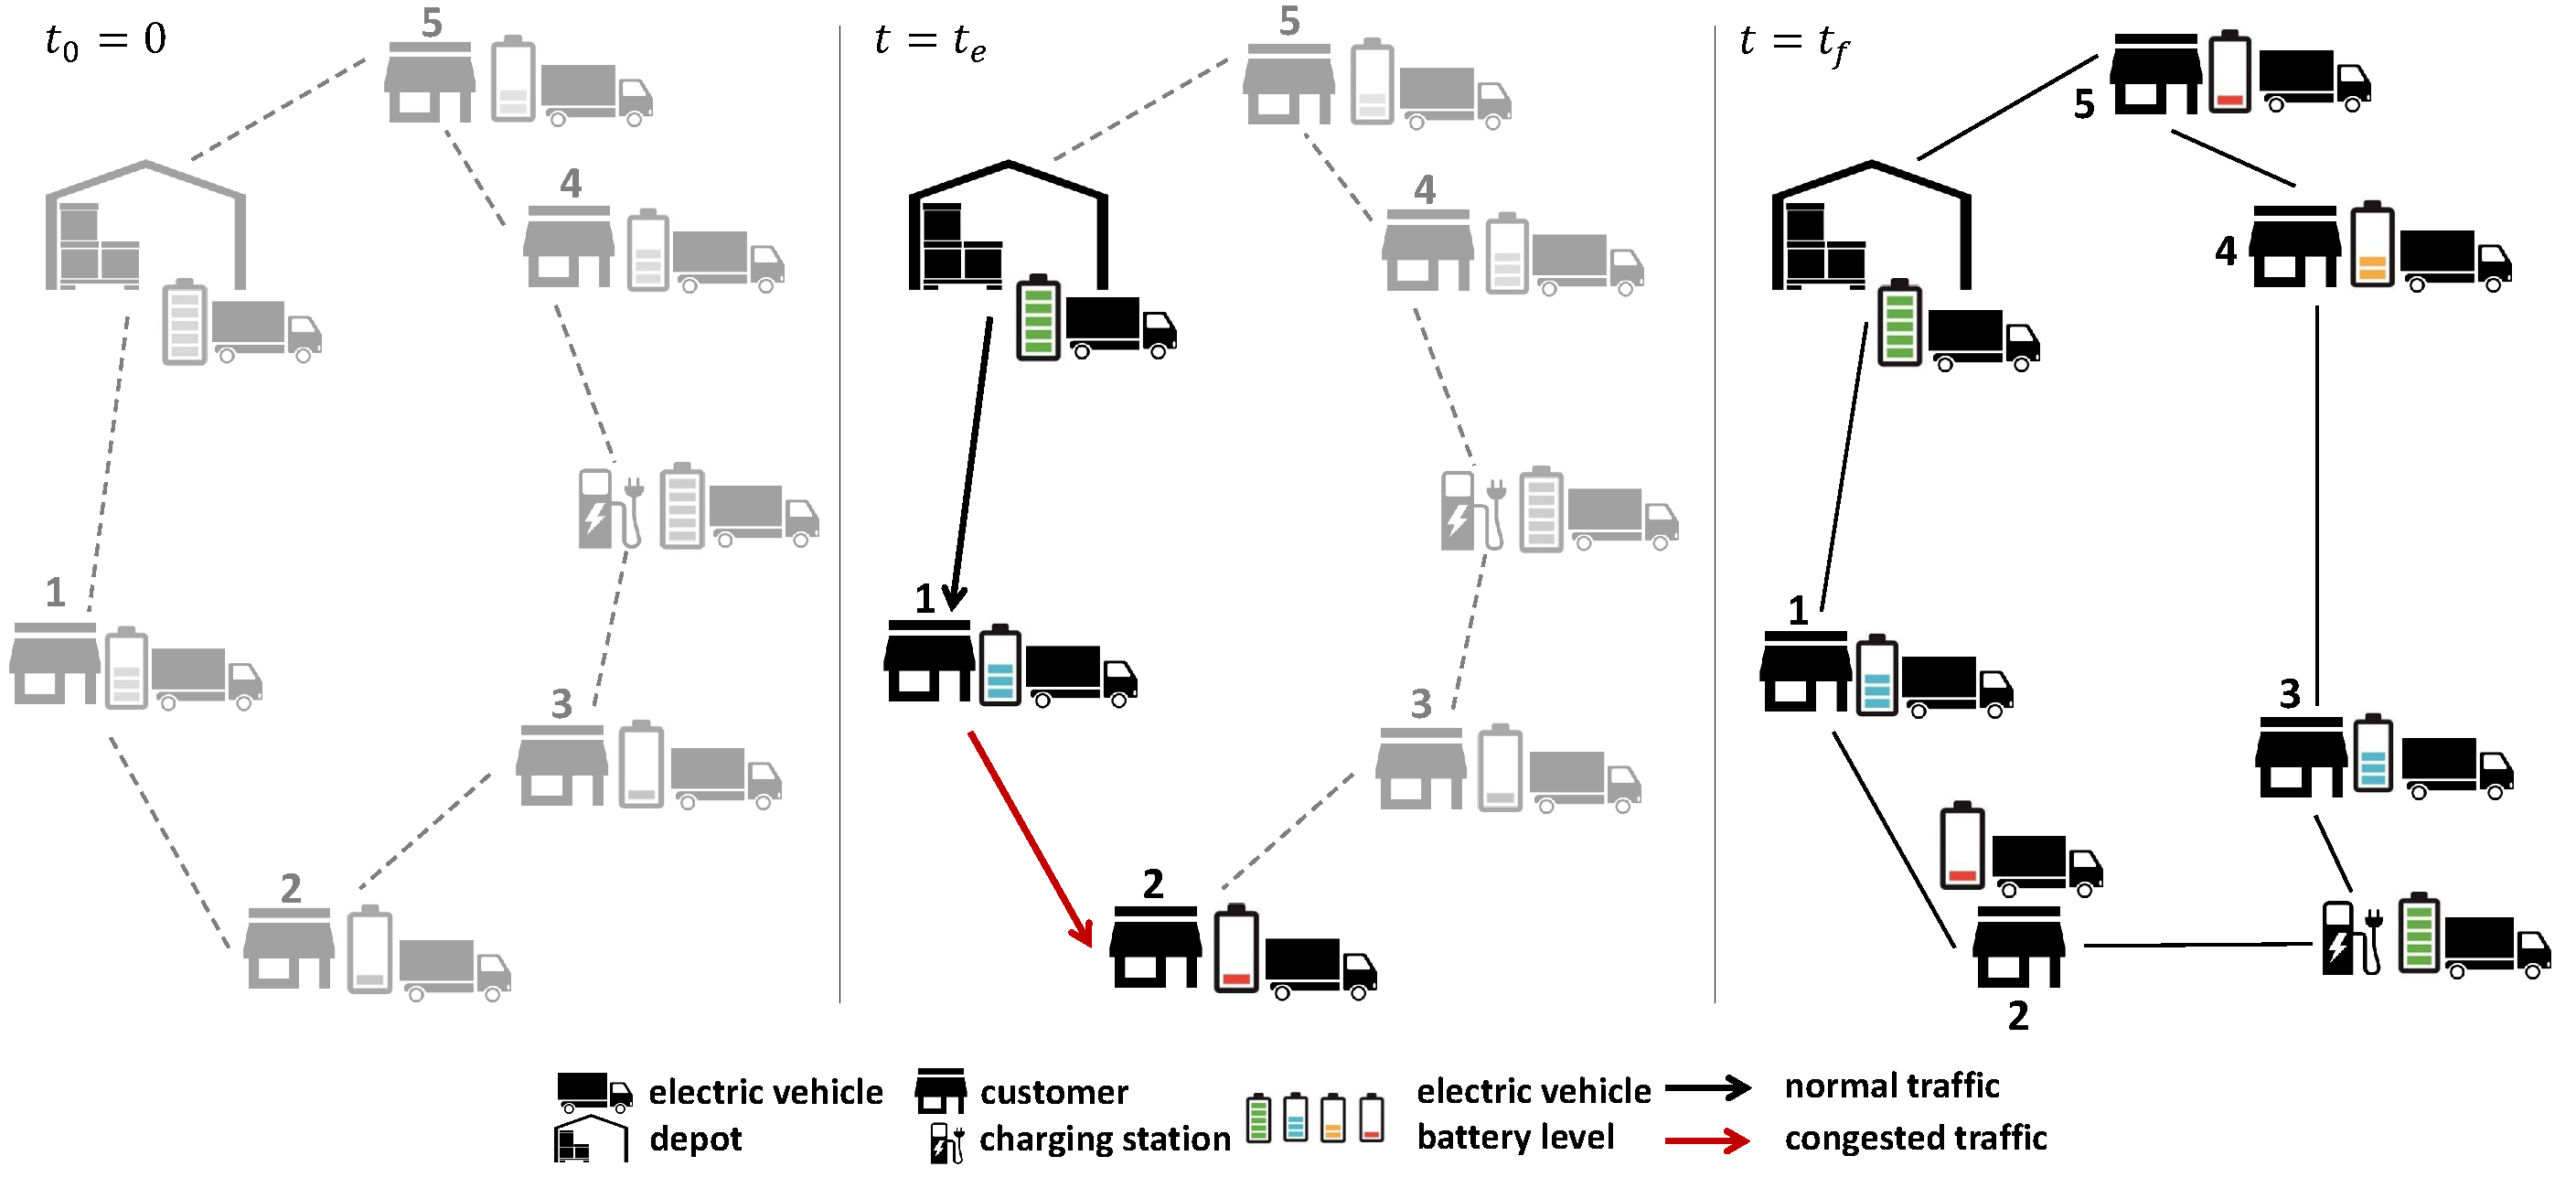
\includegraphics[width=1\linewidth]{Figure1.pdf}
    \caption{Example of the Dynamic electric vehicle routing problem under uncertainties}
     \label{Fig1}
     \end{centering}
\end{figure}

%%%%%%%%%%%%%%%%%%%%%%%%%%%%%%%%%%%%%%%%%%%%%%%%%%%%%%%%%%%%%%%%%%%%%%%%%%%%%%%%
\section{Static heterogeneous electric vehicle routing problem under uncertainties}
\label{section:model}
%%%%%%%%%%%%%%%%%%%%%%%%%%%%%%%%%%%%%%%%%%%%%%%%%%%%%%%%%%%%%%%%%%%%%%%%%%%%%%%%
As mentioned before, the DHEVRP can be studied from two perspectives. In this study, we adopt a dynamic approach for dealing with the problem. We divide the time horizon in a number of stages such that the number of stages is equal to the number of times a new event occurs. At each stage, we define an static DHEVRP with the deterministic inputs and stochastic inputs. Thus, the objective of this section is to formally introduce the static DHEVRP. We first provide the definitions and notations together with some assumptions used in the model. After that, we introduce the mathematical formulation of the static problem.

 %%%%%%%%%%%%%%%%%%%%%%%%%%%%%%%%%%%%%%%%%%%%%%%%%%%%%%%%%%%%%%%%%%%%%%%%%%%%%%%%
\subsection{Problem description}
%%%%%%%%%%%%%%%%%%%%%%%%%%%%%%%%%%%%%%%%%%%%%%%%%%%%%%%%%%%%%%%%%%%%%%%%%%%%%%%%
The goal of the DHEVRP is to find a route plan to attend a set of customers with a given heterogeneous vehicle fleet while minimising acquisition costs, total travel times, and charging times. This problem is represented on a fully connected directed graph $G = (N, A)$, where $N = (0,1, 2, 3 \dots n)$ is the set of nodes and $A = \{(i, j) |  i, j \in N, i \neq j \}$ is the set of arcs. Therefore, there are $|A| = n.(n-1)$ arcs in the graph. The set of nodes is partitioned into a set of customers $C = (0,1, 2, 3 \dots c)$ and a set of dummy nodes $E'$, i.e. $N = C \cup U'$, where $U'$ contains multiple charging stations of $U = (u_1, u_2, u_3, \dots u_u)$. Let $n_0$ and $n_{n+1}$ represent the start and end depot nodes, respectively. For simplicity, we defined $N_0$ as the set of nodes with the start depot node and $N_{n+1}$ as the set of nodes with the end depot node. $N_{0, n+1}$ portrays $N \cup \{n_0, n_{n+1}\}$. We also adopt this notation for the sets $C$ and $U'$ \citep{Hiermann2016}.

Since the availability of each charging station $i \in E$ is uncertain, we represented it by a stochastic variable $\Lambda_i$, i.e. $\Lambda_i:\Gamma_{i} \to \mathbb{R}_0^+ \forall i \in N$ with sampling spaces $\Gamma_{i}$. When a vehicle arrives at node $i$ and the station is available, then $\Lambda_i = 1$. In this case, the vehicle is promptly recharged. If the station is not available, i.e. $\Lambda_i = 0$, the vehicle has to wait a time interval $w_i$ until the charging station turns available. This time interval is also uncertain, i.e. $w_i:\alpha_{i} \to \mathbb{R}_0^+ \forall i \in N$ with sampling space $\alpha_{i}$. 

The deterministic amount of goods that has to be delivered to (or/and collected at) customer $i \in C$ is denoted as customer demand and is given by $d_i$, therefore, $d_0 = 0$. Each node $i \in N$ has a time window $[e_i, l_i]$ and a service time $s_i$. The true start of the service time is stored in $\tau_i$.

There is a fleet of $K = \{1,2,...,k\}$ types of electric vehicles. For each vehicle type $k$, the variable $g^k$ expresses the charging rate (time/energy unit) and the variable $e^k$ expresses the battery energy consumption rate (energy unit/ kilometre). The maximum capacity of vehicle type $k$ is defined as $Q^k$, and $q^k_i$ displays the current load of a vehicle type $k$ in node $i$. The maximum energy capacity of vehicle type $k$ is represented by $Y^k$, and $y^k_i$ displays the remaining battery energy level of vehicle type $k$ at node $i$. The remaining battery energy level is also uncertain and it is thus represented by $y^k_i:\vartheta^k_{i} \to \mathbb{R}_0^+ \forall i \in N, \forall k \in K$ with sampling spaces $\vartheta^k_{i}$. It is worth mentioning that the time spent by EV type $k$ at a CS, that is $s_i, \forall i \in Q$, depends on the charging rate $g^k$ of vehicle type $k$, its maximum energy capacity $Y^k$, and battery energy level of the vehicle when it reaches node $y^k_i, i \in R$, i.e. $s_i= g^k(Y^k - y^k_i)$.


If an` EV type travels from $i$ to $j$, the remaining battery level at customer $y^k_j$ is calculated based on the battery level at node $i$ and en-route energy consumption. We follow the work of \cite{Felipe2014} and assume that the en-route energy consumption (expressed in KWh per km) is proportional to the distance $c_{ij}$ traveled through a given coefficient energy consumption $e^k$ for EV type $k$.

The target battery level of an EV is determined based on the estimation of energy consumption on the remainder of its route. That is to say, instead of recharging the battery from empty-to-full, top-up chargings are done. The battery is charged to a level so that the EV is able to attend the remaining customers and return to the depot.

EXPLAIN HERE HOW MUCH THE BATTERY IS CHARGED AT ANY CS

Each arc $i,j \in A$ has two variables $c_{ij}$ and $t^k_{ij}$ associated with it. $c_{ij}$ is the distance between the nodes $i$ and $j$, and $t^k_{ij}$ represents the travel time spent by vehicle type $k$ in arc $i,j$.  Travel times is represented by a stochastic variable, that is $t_{ij}:\Omega_{ij} \to \mathbb{R}_0^+ \forall i,j \in N$ with sampling spaces $\Omega_{ij}$.

Note that an instance of the problem is defined by a complete weighted graph $G = (N, A, (c_{ij},t^k_{ij}))$ together with the $|K|$ types of electric vehicles. $\alpha^k$ is defined as the acquisition cost of vehicle type $k$. The decision variables $x^k_{ij}$ indicate whether or not vehicle type $k$ travels from node $i$ to node $j$. A solution $z = \{r_1, r_2, r_3, r_k\}$ to the DHEVRP, i.e. a route plan, consists of $k$ routes. The total time is expressed by $J(z)$. A feasible route $r_k$ is performed by one electric vehicle of type $k$ which leaves the depot with a fully charged battery, serves a subset $B = \{i_1, i_2, \dots, i_b\} \subseteq C$ of customers, whose total demand does not exceed $Q^k$, recharges its battery at a charging station $u \in U'$ if necessary, and returns to the depot, i.e. $r_k = (n_0, \gamma^k_1, \gamma^k_2, u^k_u, \dots \gamma^k_b, n_{n+1})$. 


%%%%%%%%%%%%%%%%%%%%%%%%%%%%%%%%%%%%%%%%%%%%%%%%%%%%%%%%%%%%%%%%%%%%%%%%%%%%%%%%
\subsection{Mathematical model}
%%%%%%%%%%%%%%%%%%%%%%%%%%%%%%%%%%%%%%%%%%%%%%%%%%%%%%%%%%%%%%%%%%%%%%%%%%%%%%%%
The static DHEVRP is presented as a three-index mixed integer programming model:
\begin{align}
		\label{Problem:CVRP}
		\underset{z}{\text{min }} & J(z) := \min \sum_{k \in K}\sum_{i \in N_{0}, j \in N_{n+1} i \neq j}E[t^k_{ij}]x^k_{ij} + \sum_{i \in U'}E[s_i] + \sum_{i \in U'}E[w_i|\Lambda_i = 0] \displaybreak[0]\\ 
		\label{Problem:CVRP1}
		\text{s.t. } &\sum_{k \in K}\sum_{j \in N_{n+1}, i \neq j}x^k_{ij} =1, \qquad \forall i \in C \displaybreak[0]\\
		%
		\label{Problem:CVRP2}
		&\sum_{k \in K}\sum_{j \in N_{n+1}, i \neq j}x^k_{ij} \leq 1, \qquad \forall i \in R' \displaybreak[0]\\
		%
		\label{Problem:CVRP3}
		&\sum_{i \in N_{n+1}, i \neq j}x^k_{ji} - \sum_{i \in N_{0}, i \neq j}x^k_{ij} = 0, \qquad \forall j \in N, \forall k \in K
 \displaybreak[0]\\
		%
		\label{Problem:CVRP4}
		&e_j \leq E[\tau_j] \leq l_j, \qquad \forall j \in N_{0,n+1} \displaybreak[0]\\
		%
		\label{Problem:CVRP5}
		&E[\tau_i] + (E[t_{ij}] + s_i)x^k_{ij} - l_0(1-x^k_{ij}) \leq E[\tau_j], \qquad \forall k \in K, \forall i \in C_0, \forall j \in N_{n+1}, i \neq j \displaybreak[0]\\
		\label{Problem:CVRP6}
		&E[\tau_i] + E[t^k_{ij}]x^k_{ij} + g^k(Y^k - y^k_i) - (l_0 + g^kY^k)(1-x^k_{ij}) \leq E[\tau_j], \quad \forall K \in K, \forall i \in U', \forall j \in N_{n+1}, i \neq j \displaybreak[0]\\
		\label{Problem:CVRP7}
		& q^k_j \leq q^k_i - d_i x^k_{ij} + Q^k(1+x^k_{ij}), \qquad \forall k \in K, \forall i \in N_{0}, \forall j \in N_{n+1}, i \neq j \displaybreak[0]\\
		\label{Problem:CVRP8}
		&0 \leq q^k_j \leq Q^k, \qquad \forall k \in K, \forall j \in N_{0,n+1}\displaybreak[0]\\
		\label{Problem:CVRP9}
		&0 \leq y^k_j \leq y^k_i - (E[e^k] d_{ij})x^k_{ij} + Y^k(1 - x^k_{ij}), \qquad \forall k \in K, \forall i \in C, \forall j \in N_{n+1}, i \neq j\displaybreak[0]\\
		\label{Problem:CVRP10}
		&0 \leq y^k_j \leq Y^k - (E[e^k] d_{ij})x^k_{ij}, \qquad \forall k \in K, \forall i \in U'_{0}, \forall j \in N_{n+1}, i \neq j \displaybreak[0]\\
		\label{Problem:CVRP11}
		&y^k_0 = Y^k \qquad \forall k \in K\displaybreak[0]\\
		\label{Problem:CVRPbinary}
		& x^k_{ij} \in \{0, 1\} \qquad \forall i \in N_0, j \in N_{n+1}, i \neq j, \forall k \in K
\end{align}

This is a minimization problem with an objective function \eqref{Problem:CVRP} that consists of XXXX terms. The XXXX and XXXX terms are the total travel time and the total charging time, respectively. According to \cite{Montoya2017}, by including the sum of the charging time in the objective function, one can capture better the impact of charging operations. The XXXX term counts the total waiting time at charging stations. This is particular important when the availability of charging stations is uncertain and the vehicles have, therefore, to wait before being recharged. Constraints \eqref{Problem:CVRP1} assure that each customer is visited by one incoming and one outgoing vehicle. Constraints \eqref{Problem:CVRP2} mean that a charging station is visited at most once and that it does not necessary need to be visited by a vehicle. Flow conservation is guaranteed by constraints \eqref{Problem:CVRP3}. Contraints \eqref{Problem:CVRP4} ensure that the start time of a service $\tau_i$ at a node $i$ has to be within its time window. Constraints \eqref{Problem:CVRP5} and \eqref{Problem:CVRP6} track the start time of a service and show the difference between customers and charging stations nodes regards service times. If the previous node is either a customer or the depot, constraints \eqref{Problem:CVRP5} consider the service time, while constraints \eqref{Problem:CVRP6} consider the charging time if the previous node is a charging station. The charging time of vehicle type $k$ is calculated based on its charging rate $g^k$, its maximum energy capacity $Y^k$, and its remaining battery level when it arrives at the charging station $i$ ($y^k_i$). Constraints \eqref{Problem:CVRP7} guarantee that the demand of every customer is satisfied. Vehicle capacity restrictions are expressed by constraints \eqref{Problem:CVRP8}. Constraints \eqref{Problem:CVRP9} and \eqref{Problem:CVRP10} not only trace the battey level of the vehicle type $k$ based on its energy consumption as it tours arc $i,j$ and its maximum energy capacity but also secure that its remaining battery level is always positive in any node. Constraints \eqref{Problem:CVRP11} secure that the battery level of any vehicle is full at the depot. Finally, the domain of the decision variables is defined by constraints \eqref{Problem:CVRPbinary}. 


%%%%%%%%%%%%%%%%%%%%%%%%%%%%%%%%%%%%%%%%%%%%%%%%%%%%%%%%%%%%%%%%%%%%%%%%%%%%%%%%
\section{Solution approach}
\label{section:approach}
%%%%%%%%%%%%%%%%%%%%%%%%%%%%%%%%%%%%%%%%%%%%%%%%%%%%%%%%%%%%%%%%%%%%%%%%%%%%%%%%
In this section, we describe the proposed solution approach. Our approach is based on the MSA. The key idea behind MSA is to continuously generate and solve scenarios. In MSA, online decisions are made according to a distinguished plan which evolves over time \citep{Bent2004}. Figure \ref{Fig2} displays a high level flow diagram of the proposed solution approach. It contains mainly five stages. These stages are described in the next sections.

\begin{figure}[H]
\begin{centering}
  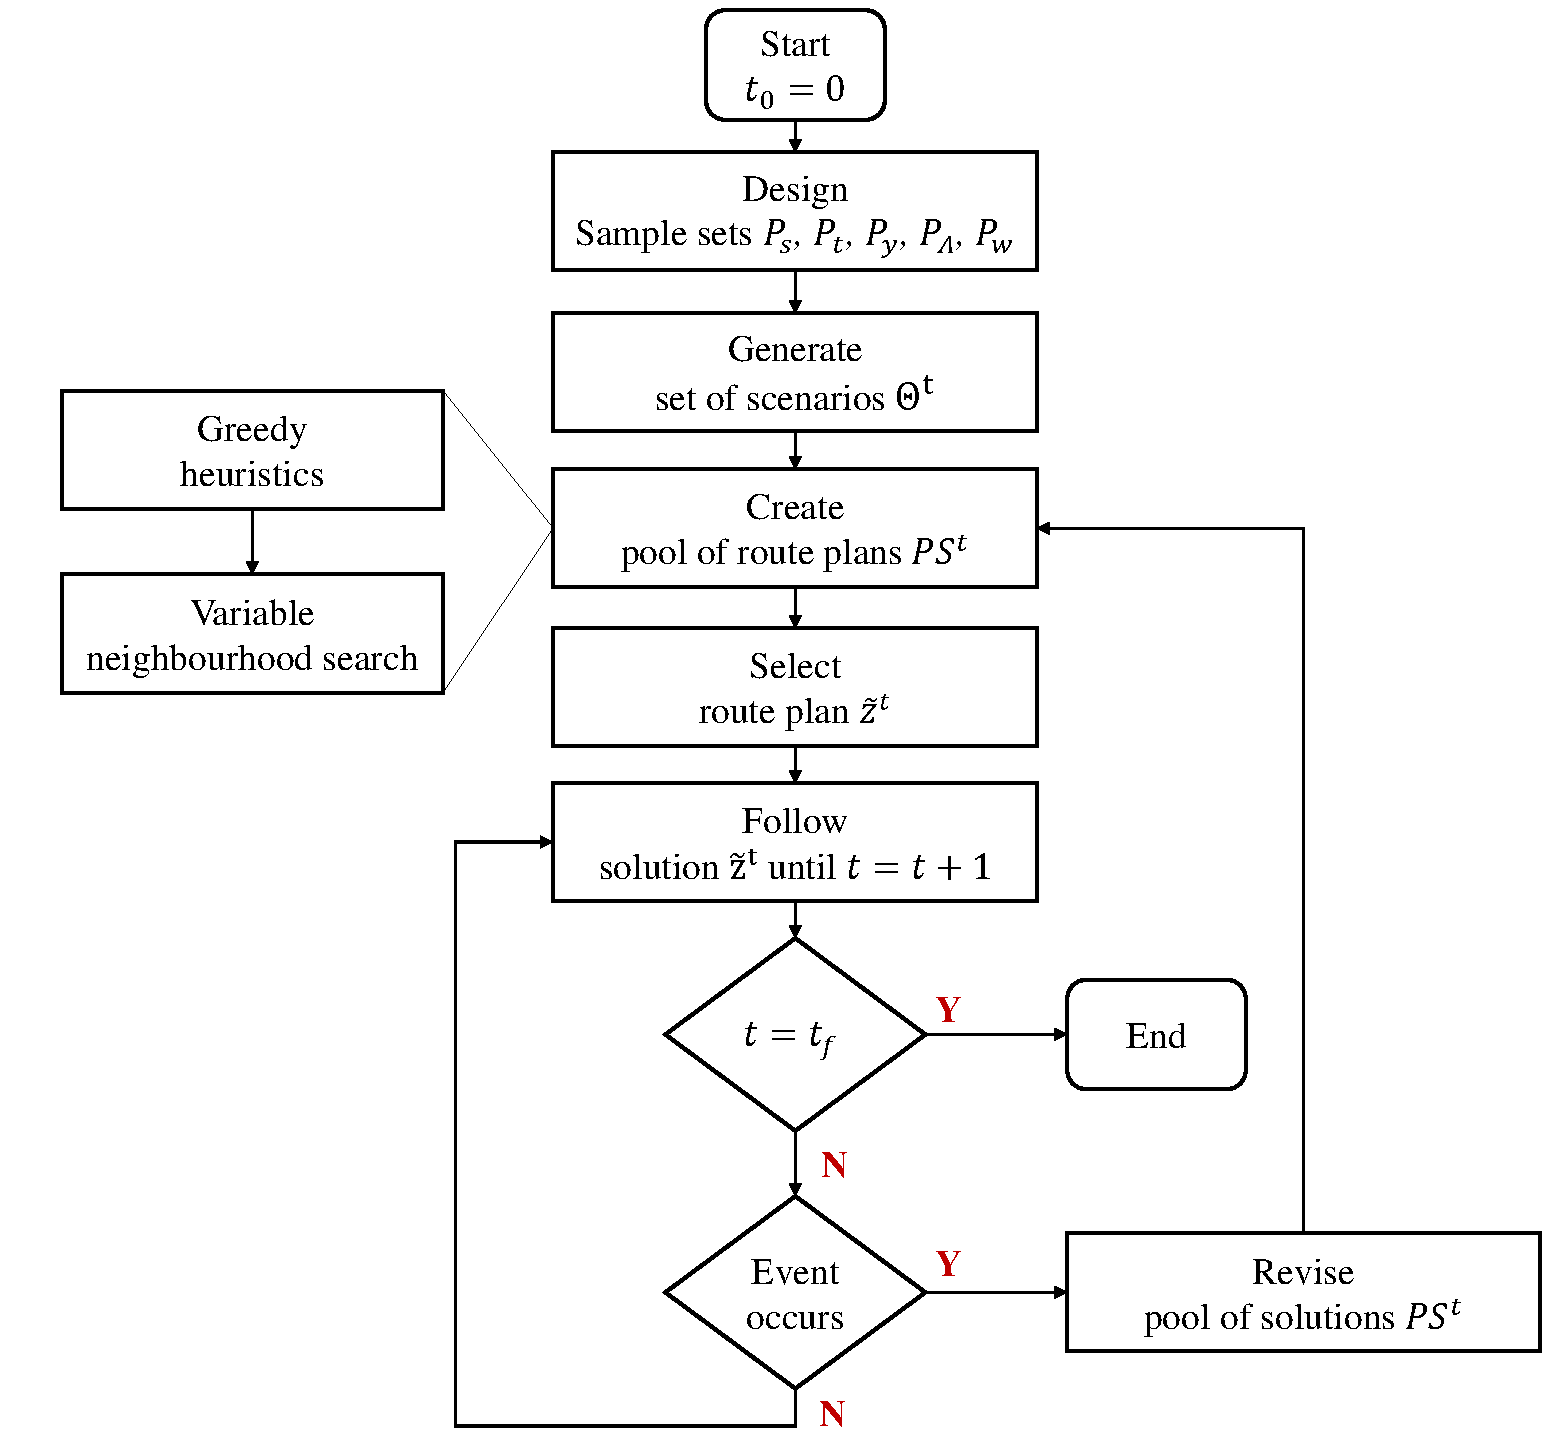
\includegraphics[width=0.79\linewidth]{Figure2.pdf}
    \caption{A dynamic approach for the DHEVRP}
     \label{Fig2}
     \end{centering}
\end{figure}

%%%%%%%%%%%%%%%%%%%%%%%%%%%%%%%%%%%%%%%%%%%%%%%%%%%%%%%%%%%%%%%%%%%%%%%%%%%%%%%%
\subsection{Stage 1: sample sets design}
\label{section:step1}
%%%%%%%%%%%%%%%%%%%%%%%%%%%%%%%%%%%%%%%%%%%%%%%%%%%%%%%%%%%%%%%%%%%%%%%%%%%%%%%%
In the first stage, we obtain one set of samples of each stochastic input by using Monte Carlo sampling and the probability distributions that model the uncertain input. Thus, five sample sets are generate
\begin{align}
	\label{eq:ss}
	P_s = \{ p^m_s = (s^m_1, s^m_2, s^m_3 \ldots, s^m_c) \mid m = 0, \ldots, \beta \},
\end{align}
\begin{align}
	\label{eq:tt}
	P_t = \{ p^m_t = (t^m_{01}, t^m_{02}, t^m_{03} \ldots, t^m_{n(n-1)}) \mid m = 0, \ldots, \beta \},
\end{align}
\begin{align}
	\label{eq:remaining}
	P_y = \{ p^m_y = (y^{1,m}_0, y^{2,m}_0, y^{3,m}_0 \ldots, y^{k,m}_0) \mid m = 0, \ldots, \beta \},
\end{align}
\begin{align}
	\label{eq:availability}
	P_{\Lambda} = \{ p^m_{\Lambda} = (\Lambda^m_1, \Lambda^m_2, \Lambda^m_3 \ldots, \Lambda^m_r) \mid m = 0, \ldots, \beta \},
\end{align}
\begin{align}
	\label{eq:waiting}
	P_w = \{ p^m_w = (w^m_1, w^m_2, w^m_3 \ldots, w^m_r) \mid m = 0, \ldots, \beta \}.
\end{align}
Sets \eqref{eq:ss}, \eqref{eq:tt}, \eqref{eq:remaining}, \eqref{eq:availability}, and \eqref{eq:waiting} represent service time, travel time, remaining battery energy level, availability of CS, and waiting time at CS sample set, respectively. A service time sample $p^m_s$ defines one value for $s_i$, $\forall i \in C$. Thus, $|p^m_s| = |C|$. In the case of the travel time sample set, a sample $p^m_t$ specifies one value for $t_{ij}$,  $\forall i, j \in A$, $i \neq j$. Hence, $|p^m_t| = |A|$.  The number of elements in $p^m_y$ differs at \textbf{Step 1} and \textbf{Step 4}. At $t_0 = 0$, all vehicles in the fleet are located at the depot ($i=0$), and there has not been en-route energy consumption. Therefore, one sample $p^m_y$ defines one value of battery energy level for each vehicle type $k$, i.e. $|p^m_y| = |K|$. We consider two cases for the battery energy level at $t_0 = 0$. These cases are described in \textbf{Section \ref{section:cases}}. On the other hand, at \textbf{Step 4}, EVs have visited different customers, so $|p^m_y| = k.|C|$. Sample $p^m_{\Lambda}$ determines one probability for each CS, while $p^m_w$ states one value for $w_i$, $\forall i \in R$. Thus, $|p^m_{\Lambda}|, |p^m_w| = |R|$. We consider three cases for the availability of CS, and consequently waiting time at CS. These cases are also described in \textbf{Section \ref{section:cases}}. 

%%%%%%%%%%%%%%%%%%%%%%%%%%%%%%%%%%%%%%%%%%%%%%%%%%%%%%%%%%%%%%%%%%%%%%%%%%%%%%%%
\subsection{Stage 2: set of scenarios generation}
\label{section:step2}
%%%%%%%%%%%%%%%%%%%%%%%%%%%%%%%%%%%%%%%%%%%%%%%%%%%%%%%%%%%%%%%%%%%%%%%%%%%%%%%%
In the second stage, the set of scenarios $\Theta^t = (\theta^t_1, \theta^t_2, \ldots , \theta^t_{\beta})$ is created. Each scenario is generated by randomly selecting one sample in every sample set, e.g. $\theta^t_{64} = (p^{50}_s, p^4_t, p^{10}_y, p^{33}_{\Lambda}, p^{27}_w, N, A)$. All the scenarios in $\Theta^t$ have the same set of nodes $N$ and set of arcs $A$. That is to say, every scenario is a deterministic instance of the stochastic problem.


%%%%%%%%%%%%%%%%%%%%%%%%%%%%%%%%%%%%%%%%%%%%%%%%%%%%%%%%%%%%%%%%%%%%%%%%%%%%%%%%
\subsection{Stage 3: pool of solutions creation}
\label{section:stage3}
%%%%%%%%%%%%%%%%%%%%%%%%%%%%%%%%%%%%%%%%%%%%%%%%%%%%%%%%%%%%%%%%%%%%%%%%%%%%%%%%
In the third stage, all $\beta$ scenarios in the set $\Theta^t$ are solved, creating the pool of solutions $PS^t = (z^t_1, z^t_2, \dots z^t_{\beta})$. Since every scenario in the set is a deterministic instance of the DHEVRP, we can make use of well-established heuristics to solve them. We adopt two heuristics to solve all the scenarios, a greedy algorithm and a randomized variable neighbourhood search (VNS). These heuristics are explained as follows.

The greedy algorithm is used to calculate the initial solution. Its pseudocode is displayed in \textbf{Algorithm \ref{algorithm:greedy}}. In this method, a customer $i \in C$ is allocated to the EV route $r^k$ that has traveled time $J(r^k)$ closer to the time window of the request $[e_i;l_i]$ (Step \ref{lst:line:minimum}). A customer's request is only added to a route when feasibility can be maintained with respect to remaining battery energy level $y^k_i$ and EV capacity $q^k_i$ . If customer $i$ cannot be added to route $r^k$ because of battery energy level feasibility (Step \ref{lst:line:batteryfeasi}), the CS $u_j \in U'$ with lowest sum of the distance to the current customer $c_{ij}$ plus waiting time $w_j$ is inserted in the EV route (Step \ref{lst:line:CSminimum}). This CS is then removed from the list of available CS (Step \ref{lst:line:removeCS}). Since we do not adopt fully charged setting, one has to decide how much to recharge when the EV stops at the CS. As explained before, in this paper we follow that the decision on how much to recharge the battery of any EV at any CS is based on the rest of the customers to be attend by this EV. Nevertheless, this procedure is impracticable at this stage. The initial route plan is being constructed, and not all the customers have, therefore, been assigned to the EVs. We thus create three scenarios that will guide this decision during the creation of the initial route plan. These scenarios are described in \textbf{Section \ref{section:cases}}. If customer $i$ cannot be allocated to route $r^k$ due to capacity feasibility (Step \ref{lst:line:capacityfeasi}), the EV returns to the depot and it is removed from the list of available EVs (Step \ref{lst:line:removeEV}). The greedy method repeats these steps until all the customers are designated to EV routes. The solution outputed by the greedy method $z_g$ is improved by the VNS. 

We implement a VNS modified from the VNS proposed by \cite{Mladenovic1997}. The pseudocode of the VNS is displayed in \textbf{Algorithm \ref{algorithm:VNS}}. VNS requires the determination of three components: shaking procedure, local search procedure, and stopping criteria. For the shaking procedure, a list of neighbourhood structure must be define. The list of neighbourhood structures $M = \{m_1, m_2, m_3,\ldots, m_{max}\}$ is a finite set of neighbourhood structures whose $m_1(z')$, for instance, is the set of solutions in the $1^{st}$ neighbourhood of the solution $z'$. To define a neighbourhood of the solution $z$ a combination of operators must be specified. We create a list of four operators $O = \{o_1, o_2, o_3, o_4\}$. The $o_1$ (1-0 exchange move) operator removes a customer from its original route and inserts it after other in a different route. The $o_2$ (1-1 exchange move) operator swaps two customers in the same route, whereas the $o_3$ (2-opt move) operator swaps two customers in different routes. The $o_4$ (CROSS-exchange) \citep{Taillard1997} operator exchanges two arcs of different routes. All operators are used to determine the set of neighbourhood structures $M$. We use the randomized variable neighborhood descent (RVND) method \citep{Hansen1997} as the local search procedure and define the number of iterations ($iterMax$ = 1000) without improvement on the current solution as the stop criteria. VNS starts by generating a neighbour $z^a$ of the incumbent solution $z'$ at random from the $k^{th}$ neighbourhood ($z^a \in m_k(z')$). Following, the local procedure is applied to improve the solution $z^a$. In order to do so, the RVND uses a list of neighbourhood structures $V = \{v_1, v_2, v_3, \ldots , v_{max}\}$. First, one neighbourhood structure is randomly selected (Step \ref{lst:line:selectV}).
After that, the best solution in this neighbourhood structure $z^b$ is found by using the strategy first improvement (Step \ref{lst:line:descendent}). If $z^b$ is better than the solution $z^a$ (Step \ref{lst:line:test}), then $z^b$ is returned as the best solution. If not, this neighborhood structure is removed from the list (Step \ref{lst:line:removeV}). This procedure is executed until the list $V$ becomes empty. If the best solution found in the local procedure is not better than the imcumbent solution $z'$, VNS starts again with a new neighbourhood structure. These steps are repeated until the stop criteria is met.  

\begin{algorithm}
\textbf{INPUT:} $N, A, K$\\
\textbf{OUTPUT:} $z_g$
\begin{algorithmic}[1]
\STATE{Initialize $r^k$} 
\STATE{$G \gets C, H \gets U', I \gets K, z_g = \emptyset, \gamma^k_1 = 0$ and $J(r^k) = 0$  $\forall k \in K$, $position = 1$}
\WHILE {$G \neq \emptyset$}
	\STATE $position = position + 1$
	\STATE{Select customer $i \in C$ and EV type $k \in K$ based on $[e_i;l_i]$ and $J(r^k)$} \label{lst:line:minimum}
	\IF{$y^k_i \leq 0$} \label{lst:line:batteryfeasi}
			\STATE{Compute $c_{\gamma_{(position-1)}j}$ and $w_j$ $\forall j \in H$}
			\STATE{Select $u_j \in U$ with lowest $c_{\gamma_{(position-1)}j} + w_j$} \label{lst:line:CSminimum}
			\STATE{Allocate $u_j$ to $r^k$, $J(r^k) = J(r^k) + c_{\gamma_{(position-1)}j} + w_j$}
			\STATE{$H \gets H \backslash \{u_j\}$} \label{lst:line:removeCS}
			\STATE{Recharge battery of EV $k$ according to chosen scenario}
	\ELSIF{}
		\IF{$q^k_i \leq 0$} \label{lst:line:capacityfeasi}
			\STATE{Go to the depot, $\gamma_{position} \gets 0$, $position \gets 0$}
			\STATE{Add route $r^k$ to route plan $z_g$}
			\STATE{$I \gets I \backslash \{k\}$} \label{lst:line:removeEV}
		\ELSIF{}
			\STATE{Allocate customer $i$ to $r^k$, $\gamma_{position} \gets i$, $J(r^k) = J(r^k) + c_{(\gamma_{position-1})\gamma_{position}}$}
			\STATE{$G \gets G \backslash \{i\}$}
		\ENDIF
	\ENDIF
\ENDWHILE
\end{algorithmic}
\caption{Greedy algorithm}
\label{algorithm:greedy}
\end{algorithm}


\begin{algorithm}
\textbf{INPUT:} $z_{g}, N, A, K$\\
\textbf{OUTPUT:} $z$
\begin{algorithmic}[1]
\STATE{Initialize $M$, $O$, $V$} 
\STATE{$z_{best} \gets z_{g}, z' \gets z_{g}$}
\WHILE {$iterMax \leq 1000$}
	\STATE $k \gets 1$
	\FOR{$k = 1$ to $max$}
			\STATE{Generate a solution $z^a$ of $z'$ at random in $m_k(z)$}
			\WHILE{$V \neq \emptyset$}
			\STATE $l \gets U[1; |V|]$ \label{lst:line:selectV}	
				\STATE{Find the best solution $z^b$ in $v_l(z^a)$ via descendent method} \label{lst:line:descendent}
					\IF{$J(z^b) \leq J(z^a)$} \label{lst:line:test}
						\STATE{$z^a \gets z^b$}
						\STATE{$z_{best} \gets z^a$}
						\ELSIF{}
							\STATE{$V \gets V \backslash \{v_l\}$} \label{lst:line:removeV}
					\ENDIF
			\ENDWHILE
			\IF{$J(z') \leq J(z_{best})$}
				\STATE$z_{best} \gets z'$
				\STATE $iterMax = iterMax + 1$
				\STATE $k = k + 1$
			\ELSIF{}
				\STATE$z' \gets z_{best}$
			\ENDIF
	\ENDFOR
	\STATE$z \gets z_{best}$
\ENDWHILE
\end{algorithmic}
\caption{Variable neighbourhood search}
\label{algorithm:VNS}
\end{algorithm}


%%%%%%%%%%%%%%%%%%%%%%%%%%%%%%%%%%%%%%%%%%%%%%%%%%%%%%%%%%%%%%%%%%%%%%%%%%%%%%%%
\subsection{Stage 4: route plan selection}
\label{section:stage4}
%%%%%%%%%%%%%%%%%%%%%%%%%%%%%%%%%%%%%%%%%%%%%%%%%%%%%%%%%%%%%%%%%%%%%%%%%%%%%%%%
In this stage, we select the solution to be followed by the electric vehicles to attend all the customers. After the pool of route plans is created, the route plan with the smallest objective function \eqref{Problem:CVRP} value $\tilde{z}^t$ is selected out of the pool $PS^t$ at each time $t$. The route plan $\tilde{z}^t$ is then followed by the electric vehicles until a new event occurs.

%%%%%%%%%%%%%%%%%%%%%%%%%%%%%%%%%%%%%%%%%%%%%%%%%%%%%%%%%%%%%%%%%%%%%%%%%%%%%%%%
\subsection{Stage 5: solution pool revision}
%%%%%%%%%%%%%%%%%%%%%%%%%%%%%%%%%%%%%%%%%%%%%%%%%%%%%%%%%%%%%%%%%%%%%%%%%%%%%%%%
When an event occurs the pool of solutions must be revised. The possible events are described in the following. Although each event is solely explained, many of them can happen at the same time. 

\begin{itemize}
\item \textbf{Electric vehicle arrival at customer.} 
When an electric vehicle type $k$ arrives at customer $j \in C$ coming from node $i \in N$, the true values of two stochastic inputs are disclosed: travel time and remaining battery energy level.
\item \textbf{Electric vehicle arrival at charging station.}
Apart from the true values of the travel time and remaining battery level, the real availability of the CS is also revealed when an EV type $k$ arrives at charging station $i \in U$ coming from customer $i \in C$. 
\item \textbf{Electric vehicle departure from a charging station.}
The true values of both the waiting time $w_i$ and the charging time $s_i$ are disclosed when an EV departures from a charging station $i \in U$. 
\end{itemize}

The pool $P^t$ is updated by removing the route plans that are incompatible with the current system status. For instance, if route plan $\tilde{z}^t$ specifies that EV type $k$ must proceed to customer $j$ after visiting customer $i$, but the event \textbf{electric vehicle arrival at customer} $i$ shows that the remaining battery level is not enough to reach customer $j$, all solutions in $P^t$ that determine the arrival at $j$ after $i$ are deleted from the pool. Since the solution approach always keeps $\beta$ solutions in the pool at each time $t$, the same amount of deleted solutions must be created. For updating the pool, first the sample sets and then the set of scenarios $\Theta^t$ must be updated, i.e. the solution approach return to \textbf{Stage 1}. It is important to mention that the stochastic inputs that have been disclosed before $t$ do not need to be sampled again in \textbf{Stage 1} at time $t$. 



%%%%%%%%%%%%%%%%%%%%%%%%%%%%%%%%%%%%%%%%%%%%%%%%%%%%%%%%%%%%%%%%%%%%%%%%%%%%%%%%
\section{Dataset design}
\label{section:dataset}
%%%%%%%%%%%%%%%%%%%%%%%%%%%%%%%%%%%%%%%%%%%%%%%%%%%%%%%%%%%%%%%%%%%%%%%%%%%%%%%%
We evalute the performance of our solution approach in set of instances adapted from the dataset of \cite{Solomon1987}. We also compare our dynamic solution approach with a static solution approach in terms of quality of the solutions and computational time. Our dataset contains 56 instances. The inputs number of nodes $N$, customer locations $C$, demands $d_i$, travel times $t^k_{ij}$, and service times $s_i$ are taken from these instances. For the representation of the uncertain travel times, we assume that the values defined in the Solomon's instances represent the expected values, and we randomly generate the variances. The same procedure is followed for the customer service times. 

For creating the fleet of heterogeneous electric vehicles, we select some of the EVs described in \cite{mobility2013}. Because this report does not present the charging rates of the EVs, we have to generate them. According to \citep{Montoya2017}, for a battery capacity of 22 kWh, the minimum charging time is 0.50 h, i.e. $g^k$ = 0.02. Therefore, we randomly generate the charging rates in $[0.02;0.06]$. The details of the vehicles are displayed in Table \ref{table:vehicles}.

\begin{table}[H]
	\begin{center}
	\begin{tabular}{c c c c c}
	\toprule
	Name & $Q^k$ (kg) &  $Y^k$ (kWh) & $e^k$ (kWh/km) & $g^k$ (h/kWh)\\ \midrule
	German E-Cars Pantos & 1.000 & 38,60  & 0,25 & 0.05\\
	Citro\"{e}n Berlingo &500 &23,50 &0,22 & 0.03 \\
	Mercedes Vito E-CELL & 900 & 36,00& 0,22 & 0.04\\
	Renault Kangoo Z.E. & 595 & 22,00 & 0,17 & 0.02 \\
	Renault Kangoo Rapid Maxi Z. E. & 650  & 22,00 & 0,18 & 0.02 \\
	Smith Electric Newton Edison & 3.500 & 36,00 & 0,30 & 0.04\\
	Smith Electric Newton Newton & 2.800 & 40,00 & 0,80 & 0.05 \\
	Aixam Mega Multitruck & 500 & 60,00 & 0,22 & 0.06\\
	\bottomrule
	\end{tabular}
	\end{center}
\caption{Specifications of the available electric vehicles}
\label{table:vehicles}
\end{table}

For selecting the number of charging stations $|R|$, we adopt $|R| = \floor{0,1 \cdot |N|}$. We locate charging stations at randomly drawn nodes and one additional station at the depot. For the representation of the charging station availability and consequent waiting times, we create three scenarios. These scenarios are described in \textbf{Section \ref{section:cases}}.

%%%%%%%%%%%%%%%%%%%%%%%%%%%%%%%%%%%%%%%%%%%%%%%%%%%%%%%%%%%%%%%%%%%%%%%%%%%%%%%%
\section{Cases configuration}
\label{section:cases}
%%%%%%%%%%%%%%%%%%%%%%%%%%%%%%%%%%%%%%%%%%%%%%%%%%%%%%%%%%%%%%%%%%%%%%%%%%%%%%%%  
\subsection{Scenarios based on charging strategy at construction of initial route plan}
charge to 1 (100\%) every time an EV stops at a CS
charge to 0.75 (75\%) every time an EV stops at a CS
charge to 0.50 (50\%) every time an EV stops at a CS


%%%%%%%%%%%%%%%%%%%%%%%%%%%%%%%%%%%%%%%%%%%%%%%%%%%%%%%%%%%%%%%%%%%%%%%%%%%%%%%%
\subsection{Scenarios based on charging station availability}
%%%%%%%%%%%%%%%%%%%%%%%%%%%%%%%%%%%%%%%%%%%%%%%%%%%%%%%%%%%%%%%%%%%%%%%%%%%%%%%%
For the representation of the charging station availability, we create three scenarios. In \textit{Scenario A.1}, the CS are always available and have long waiting times. The waiting times (hours) are assumed to be uniformed distributed $w_i \sim U[1,50;2,50]$. In \textit{Scenario A.2}, the CS are available half of the time and have $w_i \sim U[1,00;1,50]$. In \textit{Scenario A.3}, the charging stations are less likely to be available but have shorter waiting times ($w_i \sim U[1,50;2,50]$).


%%%%%%%%%%%%%%%%%%%%%%%%%%%%%%%%%%%%%%%%%%%%%%%%%%%%%%%%%%%%%%%%%%%%%%%%%%%%%%%%
\subsection{Scenarios based on initial setup}
%%%%%%%%%%%%%%%%%%%%%%%%%%%%%%%%%%%%%%%%%%%%%%%%%%%%%%%%%%%%%%%%%%%%%%%%%%%%%%%%
INITIAL BATTERY ENERGY LEVEL  ($t = 0$)
all values in the samples in the set of battery energy level are equal to 1 in the \textit{Scenario B.1}
In \textit{Scenario B.2}, for initializing the set of battery energy level samples, we randomly generate the values in [0.5;1] for each electric vehicle in the fleet, i.e. $y^k_0 \sim U[0.5;1]$ $\forall k \in K$ 

Two types of scenarios. In the first scenario (\textit{Scenario B.1}), the vehicles leave the depots with their batteries fully charged, whereas in the second scenario (\textit{Scenario B.2}), the batteries are not fully charged when the vehicles leave the depot. 


%%%%%%%%%%%%%%%%%%%%%%%%%%%%%%%%%%%%%%%%%%%%%%%%%%%%%%%%%%%%%%%%%%%%%%%%%%%%%%%%
\section{Computational results}
\label{section:results}
%%%%%%%%%%%%%%%%%%%%%%%%%%%%%%%%%%%%%%%%%%%%%%%%%%%%%%%%%%%%%%%%%%%%%%%%%%%%%%%%


%%%%%%%%%%%%%%%%%%%%%%%%%%%%%%%%%%%%%%%%%%%%%%%%%%%%%%%%%%%%%%%%%%%%%%%%%%%%%%%%
\section{Conclusions}
\label{section:conclusion}
%%%%%%%%%%%%%%%%%%%%%%%%%%%%%%%%%%%%%%%%%%%%%%%%%%%%%%%%%%%%%%%%%%%%%%%%%%%%%%%%

\section*{Conflict of Interest}
\label{section:Conflict}
%%%%%%%%%%%%%%%%%%%%%%%%%%%%%%%%%%%%%%%%%%%%%%%%%%%%%%%%%%%%%%%%%%%%%%%%%%%%%%%%

The authors declare that there is no conflict of interest regarding the publication of this paper.

%%%%%%%%%%%%%%%%%%%%%%%%%%%%%%%%%%%%%%%%%%%%%%%%%%%%%%%%%%%%%%%%%%%%%%%%%%%%%%%%
% BIBLIOGRAPHY
%%%%%%%%%%%%%%%%%%%%%%%%%%%%%%%%%%%%%%%%%%%%%%%%%%%%%%%%%%%%%%%%%%%%%%%%%%%%%%%%

\bibliographystyle{apa-good3}
\bibliography{References}

%%%%%%%%%%%%%%%%%%%%%%%%%%%%%%%%%%%%%%%%%%%%%%%%%%%%%%%%%%%%%%%%%%%%%%%%%%%%%%%%
%%%%%%%%%%%%%%%%%%%%%%%%%%%%%%%%%%%%%%%%%%%%%%%%%%%%%%%%%%%%%%%%%%%%%%%%%%%%%%%%
\end{document}
%%%%%%%%%%%%%%%%%%%%%%%%%%%%%%%%%%%%%%%%%%%%%%%%%%%%%%%%%%%%%%%%%%%%%%%%%%%%%%%%



